\subsection{Brief overview}

To start off, we summed up the total sales of all shops and items combined to get a feel of potential seasonal outliers as well as a general trend.

\begin{figure}[h]
  \centering
  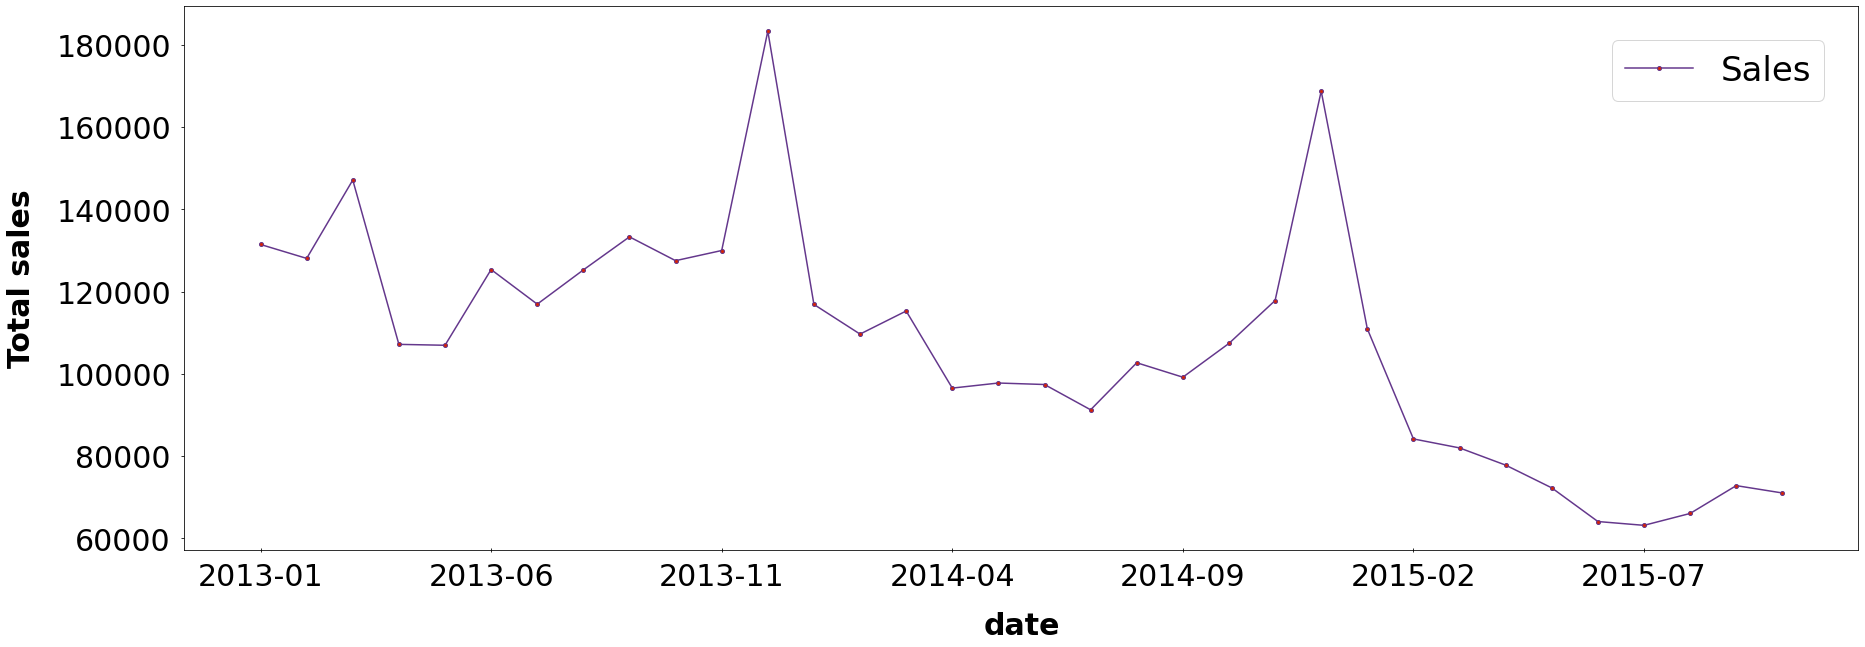
\includegraphics[width=0.9\linewidth]{external_content/graphs/total_sales.png}
  \captionsetup{justification=centering}
  \captionof{figure}{Total sales of the company}
  \label{fig:total_sales}
\end{figure}


We can observe that the sales peak in the month of December. This could be due to the increasing demand of gifts and disposable income from the population, but it could also indicate special Christmas sales which are common at this time of the year. Additionally, we observe a slight decline in demand over the timespan of the dataset.

To compare and validate the above statements, we plotted the total revenue of the company:

\begin{figure}[h]
  \centering
  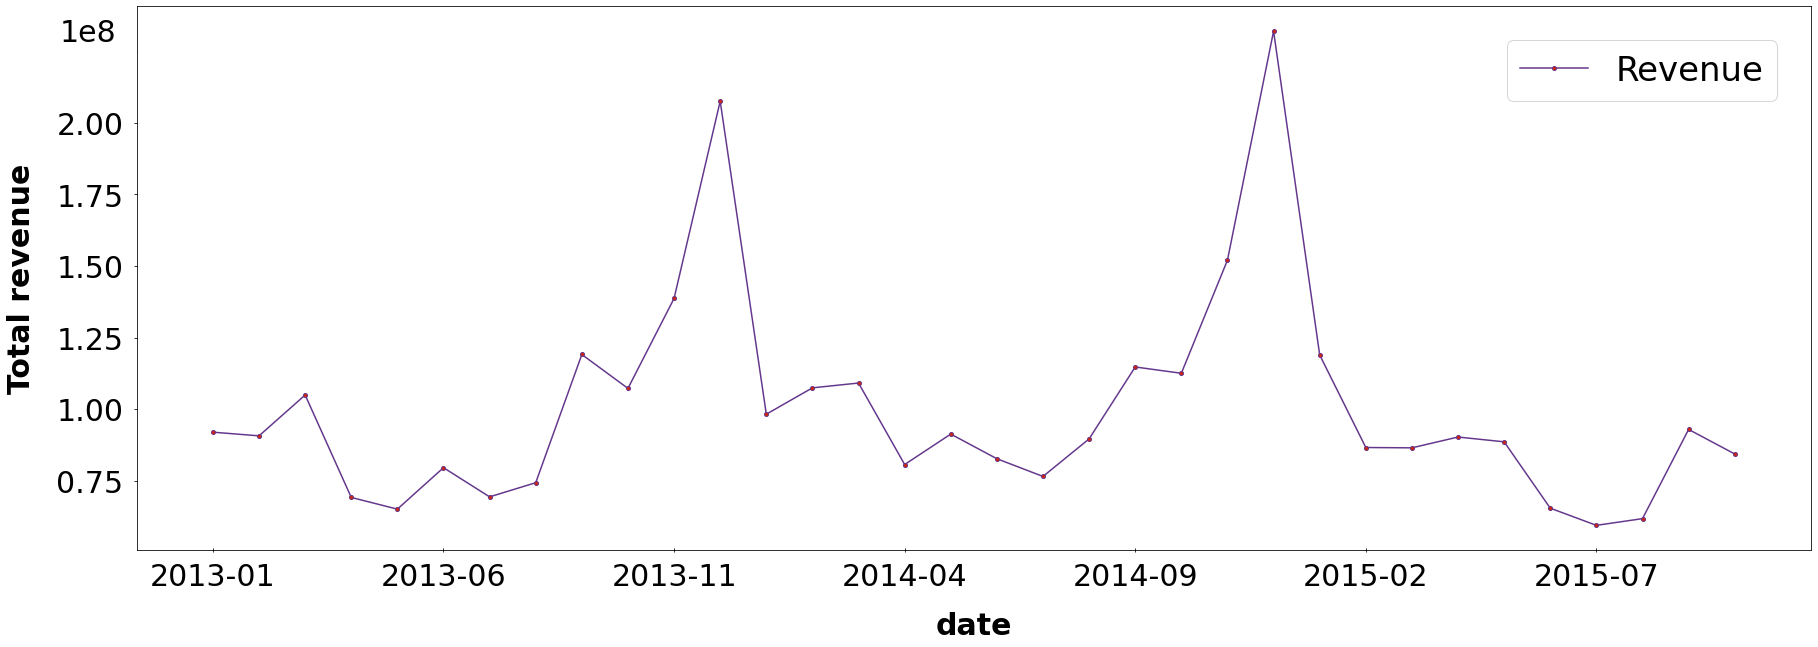
\includegraphics[width=0.9\linewidth]{external_content/graphs/total_revenue.png}
  \captionsetup{justification=centering}
  \captionof{figure}{Total revenue of the company}
  \label{fig:total_revenue}
\end{figure}

The seasonality of the data is clearly confirmed. Meanwhile, the downwards trend does not appear to be of particular relevance. The revenue stream has a constant trend over the years while having fewer sales. We should hereby be aware of the trend of having fewer sales with more expensive items.

To finish off the brief overview, we are taking a look at the correlation between the features and the label.

\begin{wrapfigure}[13]{l}{0.6\textwidth}
\centering
  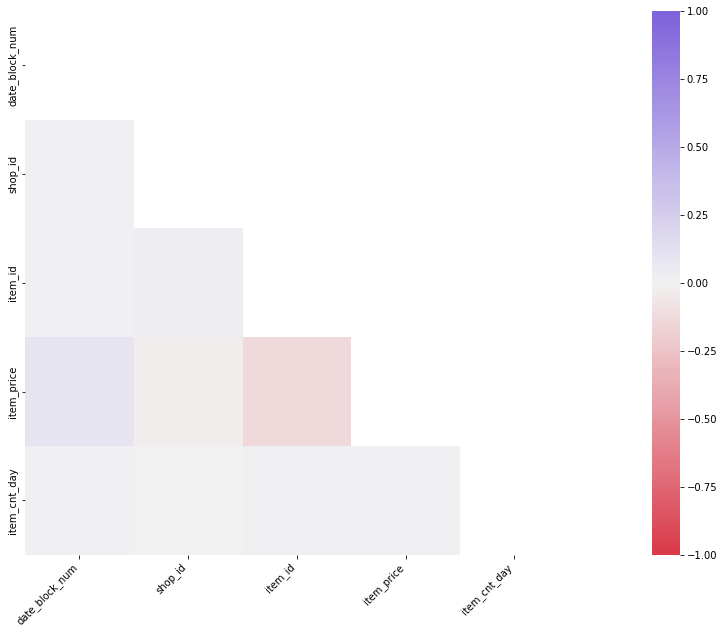
\includegraphics[width=0.85\linewidth]{external_content/graphs/corr_matrix.png}
\captionsetup{justification=centering}
\caption{Correlation matrix}
\label{corr_matrix}
\end{wrapfigure}

\noindent As we can observe, the label \texttt{item\_cnt\_day} has no strong correlation between any of the given features. 
This most likely leads to difficult to predict models, as no clear characteristics of the label is found in relation to the various features.

Additionally, no high correlation between features is observed. Therefore, we are not checking any features for multicollinearity at this point. \cite{MultivariateStatistics}

\subsection{Inspect outliers}

In this section, we are going to examine potential outliers in the training data and observe their distribution. As the \href{https://www.kaggle.com/c/competitive-data-science-predict-future-sales/overview/evaluation}{competition guidelines} suggest to clip the true target values to 20, we can savely ignore the outliers from the label as these will be clipped regardless.

\begin{figure}[h]
  \centering
  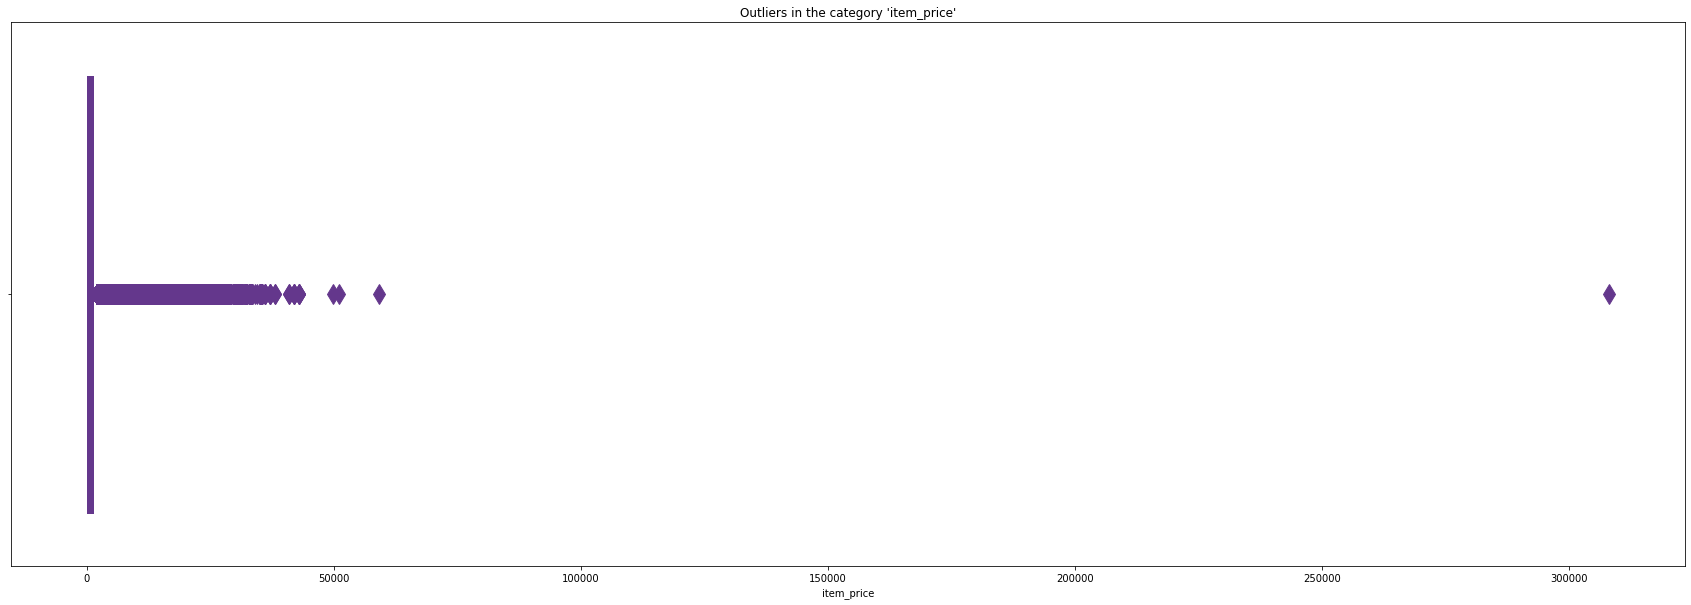
\includegraphics[width=0.9\linewidth]{external_content/graphs/outliers-item_price.png}
  \captionsetup{justification=centering}
  \captionof{figure}{Outliers of the feature \texttt{item\_price}}
  \label{fig:item_price_outliers}
\end{figure}

We can identify all but one heavy outlier from the above plot. After inspecting the outlier, we can be sure that the record is not faulty: the item in question, item nr. 6066, is a single record of a software license for 522 people.\footnote{\href{https://translate.google.com/?sl=ru&tl=en&text=Radmin\%203\%20\%20-\%20522\%20\%D0\%BB\%D0\%B8\%D1\%86.&op=translate }{Translation} - \href{https://www.radmin.com/ordering/}{Software}}

Fortunately, upon further examination, we were able to verify that the item in question is not present in the testing data and therefore not relevant for the problem.

\subsection{Distribution of sales among shops and across item categories}

We are now going to examine the distribution of the total sales in regards to the different shops as well as the different item categories. The goal is again to detect potential outliers and to get an understanding of how the sales record came about.

\begin{figure}[h]
  \centering
  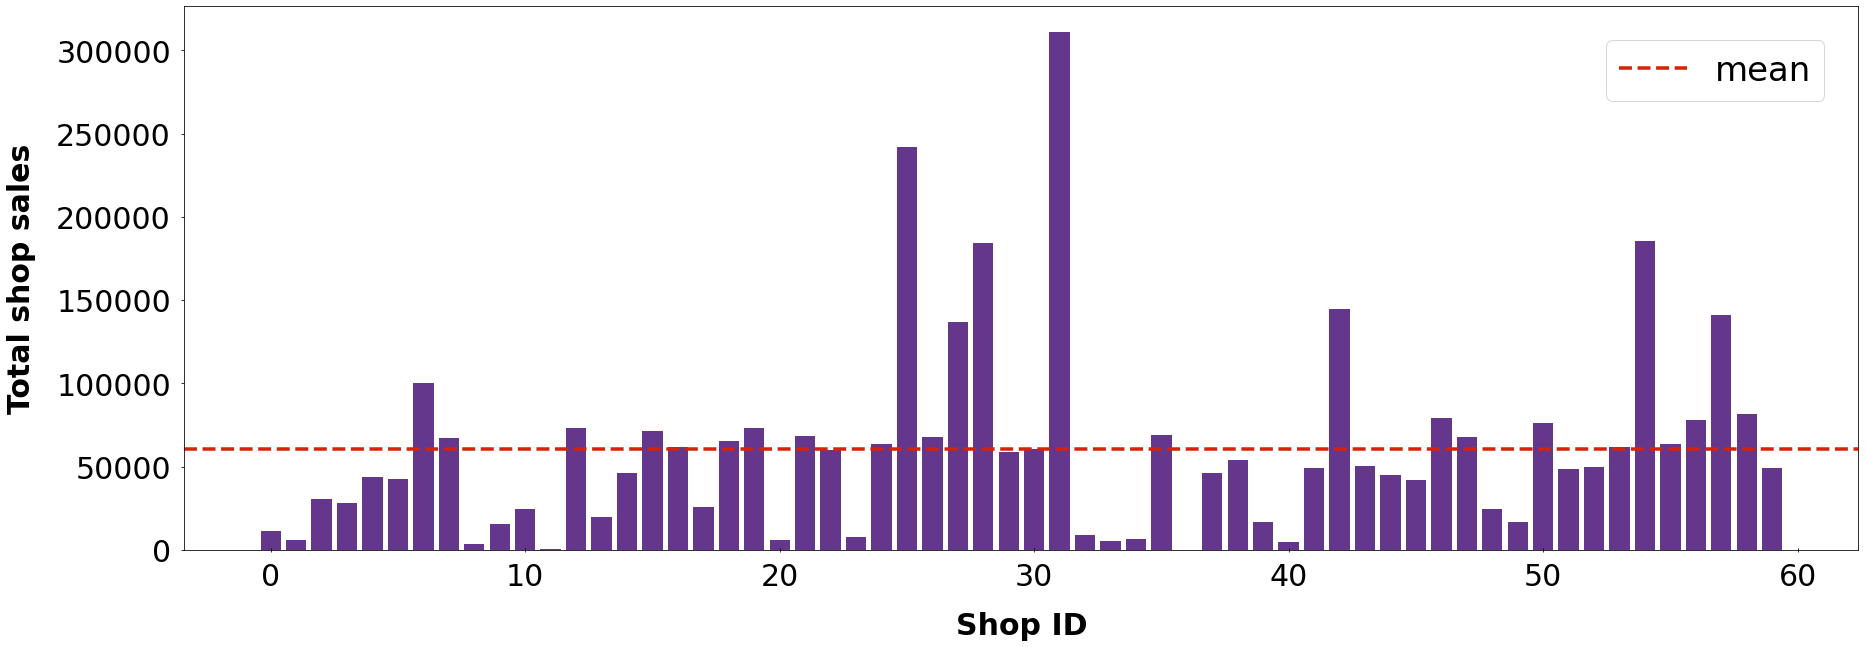
\includegraphics[width=0.82\linewidth]{external_content/graphs/distribution_amongst_shops.png}
  \captionsetup{justification=centering}
  \captionof{figure}{Distribution of total item sales across the different shops}
  \label{fig:distribution_amongst_shops}
\end{figure}

The shops in the center of the above graph appear to be very prominent. This makes sense when we take into consideration, that the shops with ID's 20--32 are all located in Moscow, the capital of the country.
The next prominent shop in the graph, shop nr. 55, is again easily understood after finding out that this is the digital shop of the company. The digital shop is common to all stores across the country which explains its high sales count.

\begin{figure}[h]
  \centering
  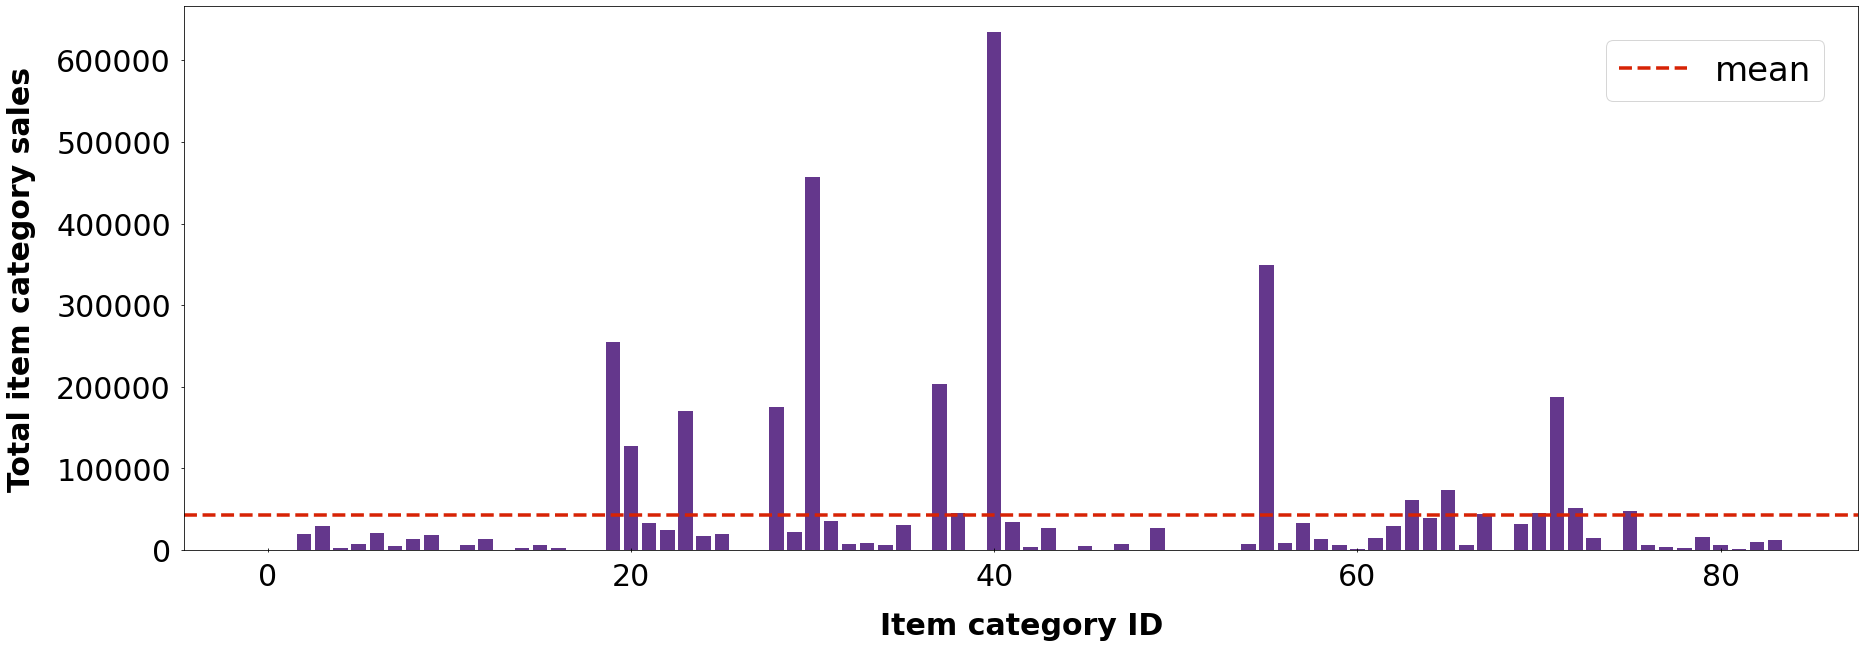
\includegraphics[width=0.98\linewidth]{external_content/graphs/distribution_across_item_categories.png}
  \captionsetup{justification=centering}
  \captionof{figure}{Distribution of total item sales within each item category}
  \label{fig:distribution_amongst_item_categories}
\end{figure}

Now, when inspecting the distribution of sales within a given item category, the space division is pretty uneven. When diving into the details, we can again relatively easily make sense as of why this came across.
The three most prominent item categories, are namely: PC Games, Movies \& Music. With the importance of the entertainment industry, these results are foreseeable.

In contrast to the best selling items, we have inspected the categories which appear to be non-existant at first glance. After making sure that no category is missing any records, the worst selling item categories are simply explained after finding out what they are all about: a mix of niche and novelty items as well as books. The lowest selling categories with less than 10 sales each are: accessories for a long outdated gaming console, games for the Apple Mac OS platform and a various categories of books.

\subsection{Understanding the test data}

The test data contains a total of $214'200$ entries to be predicted. Considering the total amount of records in the train data, the relation between $13.7$ train records per test record does not appear to be very significant anymore. This surprising low number highlights the importance of a thorough feature engineering in order to create a robust model.

Before that, we are taking a look at how the test data came about. After isolating the \texttt{shop\_id} and \texttt{item\_id} duplicates, the number $214'200$ is quickly demystified: there are $5100$ unique items and $42$ unique shops. This factors up neatly to $214'200$, which in conclusion, tells us that there are exactly $5100$ items in each and every (present) shop to be predicted.

Finally, the \href{https://www.kaggle.com/c/competitive-data-science-predict-future-sales/data}{description of the Kaggle competition} hints at us to inspect if there are any new items in the test data, which are at no point in time present in the train data. Indeed, after subtracting two sets of the total items from both datasets, we can identify that there are $363$ new items, hence a total of $363*42=15'246$ entries that have never been seen by the trained model.
